\section{Hybrid Job Placement}
\label{sec: hybrid placement}

Based on our experiments with Workloads~\Rmnum{1} and \Rmnum{2}, the ``bully" behavior is
exhibited when the dragonfly network is configured with random placement and
(progressive) adaptive routing, and there is a large gap between the
communication intensity of applications running on the network.
As shown through our experimentation, contiguous placement policies give up too
much in terms of congestion and load balance, hence being an impractical solution. 
Further, running each job with a dedicated routing policy is unrealistic, 
since routing policy is part of system configuration which can not be changed
on the fly upon job submission. 
%and the policies of some jobs (adaptive) will still interfere with others.


As a natural extension of our observations, one question that arises is \emph{whether
we can combine the merits of random and contiguous placement policies in
which each application receives the performance benefits from system load
balancing while avoiding the ``bully'' behavior.} As an initial exploration of
the question, we set up a mock hybrid job placement policy, in which less
communication-intensive jobs receive contiguous allocations to avoid the
``bully" effect, while the communication-intensive jobs are allocated randomly
in order to distribute the communication load. For Workload~\Rmnum{1}, this
means AMG gets a contiguous allocation while MultiGrid and CrystalRouter get
random allocations. Note that we do not consider challenges inherent in
designing an allocation policy for production usage, such as backfilling,
reserving large contiguous sets of nodes, determining a metric for
communication intensity, etc., preferring a restricted-scope experiment
looking at the design space of dragonfly allocation policies in light of our experimental
observations.


%\subsection{Network Performance Analysis}
%
%Hybrid placement is also coupled with three routing policies, minimal, adaptive and progressive adaptive, denoted respectively as HM, HA and HPA. As presented in section~\ref{sec: workload-1 network analysis} and~\ref{sec: workload-2 network analysis}, random placement outperforms contiguous placement in terms of network performance, the analysis in this section only focuses on the comparison between hybrid and random placement policies. 
%
%\begin{table}[ht]
%\begin{center}
%\caption{Average time spent on communication by all MPI ranks when Workload I is running on dragonfly network under hybrid placement and random placement policies.} 
%\label{tab: hyb-placement-wkld-commtime}
%\begin{tabular}{l c c c c c c }
%\toprule % Top horizontal line
%\toprule
%&\multicolumn{6}{c}{Placement and Routing Configurations} \\
%\cmidrule(l){2-7}
%          & HM & HA & HPA & RM & RA & RPA \\ % Column names row
%\midrule % In-table horizontal line
%Time(ms)  &273 &255 &255 &255 &265 &264  \\ % Content row 1
%%\midrule
%%Workload II &1747 &1991 &1991 &1791 &2367 &1965 \\
%\midrule % In-table horizontal line
%\bottomrule % Bottom horizontal line
%\end{tabular}
%\end{center}
%\end{table}
%
%Due to page limit, we only present the average communication time spent by Workload~\Rmnum{1} for the evaluation of the network performance.
%\footnote{The analysis about network traffic and saturated time are omitted in this section due to page limit.}
%As shown in Table~\ref{tab: hyb-placement-wkld-commtime}, 
%hybrid placement coupled with (progressive) adaptive routing (HA, HPA) can guarantee the same performance as random placement coupled with minimal routing (RM), thus the average workload communication time stays unchanged. 
%When hybrid placement coupled with minimal routing (HM) is in use, 
%the network performance declines  as indicated by the increasing average communication time. 
%The consecutive groups assigned to AMG results in the diminishing of network resource shared by MultiGrid and CrystalRouter, 
%causing unbalanced utilization over the network.  



%\subsection{Individual Application Analysis}

\begin{figure*}[t!]
    \centering
    \begin{subfigure}[t]{0.32\textwidth}
        \centering
        \includegraphics[height=1.3 in]{hyb-plcmt/mg/commtime}
        \caption{MultiGrid Communication Time}
        \label{fig:hyb-plcmt-mg-commtime}
    \end{subfigure}\hfill
    \begin{subfigure}[t]{0.32\textwidth}
        \centering
        \includegraphics[height=1.3 in]{hyb-plcmt/cr/commtime}
        \caption{CrystalRouter Communication Time}
        \label{fig:hyb-plcmt-cr-commtime}
    \end{subfigure}\hfill
    \begin{subfigure}[t]{0.32\textwidth}
        \centering
        \includegraphics[height=1.3 in]{hyb-plcmt/amg/commtime}
        \caption{AMG Communication Time}
        \label{fig:hyb-plcmt-amg-commtime}
    \end{subfigure}
   \caption{Application communication time. Workload~\Rmnum{1} is running with all placement and routing configurations. Methods prefixed with ``H'' represent the hybrid allocation approach.}
   \label{fig:hyb-plcmt-apps-commtime}
\end{figure*}

For the purpose of brevity, we only present the
communication time distribution of each application under all placement and routing configurations, including the hybrid placement method. These results are presented in Figure~\ref{fig:hyb-plcmt-apps-commtime}. 
As shown in Figure~\ref{fig:hyb-plcmt-mg-commtime} and~\ref{fig:hyb-plcmt-cr-commtime},
MultiGrid and CrystalRouter exhibit similar performance in both hybrid and random placement, as nodes are being placed randomly in each case.
While the performance of AMG under hybrid placement, shown in Figure~\ref{fig:hyb-plcmt-amg-commtime}, still appears to exhibit significant communication interference on account of the other applications as opposed to the best contiguous placement policies, the effects are significantly reduced compared to a random-adaptive policy. We believe this to be a result of more AMG-specific traffic occupying a smaller set of routers/groups, both reducing the probability of traffic entering them through adaptive routing and increasing the relative proportion of link utilization by AMG. Of course, this comes with the costs associated with contiguous allocation, in which AMG's traffic is less likely to load balance across multiple dragonfly groups.

%\TODO{How's this? Awesome}
These initial experiments demonstrate some degree of benefit derived from using a hybrid approach, helping to alleviate the ``bully'' effect while retaining the performance of communication-intensive applications. However, the behavior is still not ideal in this case -- AMG's communications still experience performance degradation versus the contiguous configurations. Hence, more work in this area is needed to fully understand the intricate relationships between job scheduling and system/application communication behavior to achieve optimal network utilization and application performance in high-radix networks.
